\section{Methodology and Evaluation}
\label{sec:methodology}
%\emph{\color{red}Methodology and evaluation: how do you plan to evaluate whether your hypothesis is correct?}

\subsection{Experimental Setup}
\begin{figure}[t]
      \centering
      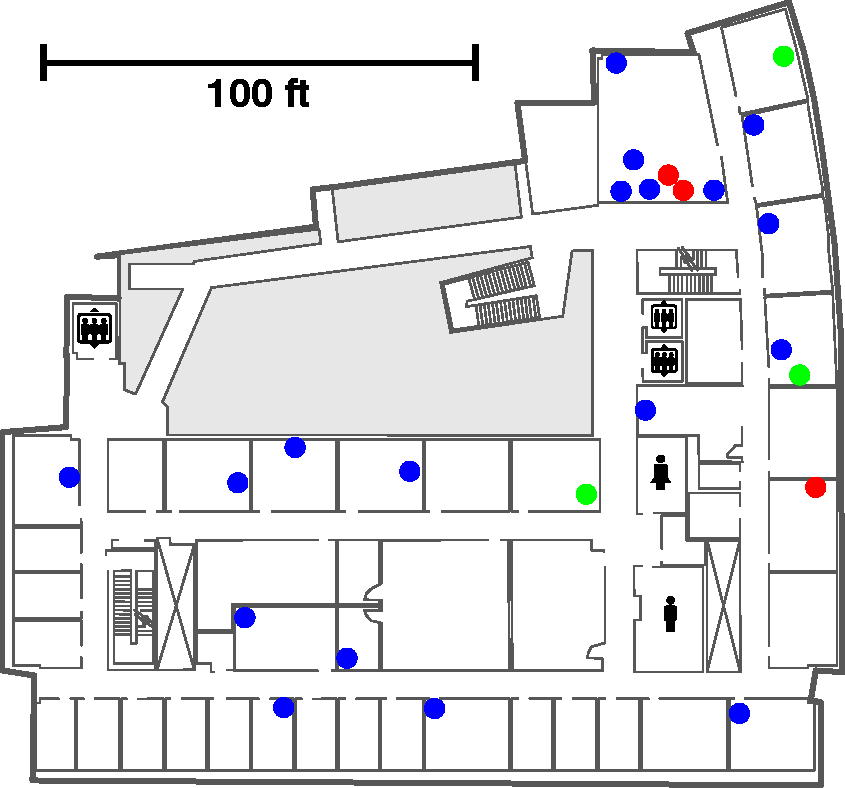
\includegraphics[width=0.8\columnwidth]{figures/floor3_grayscale_noee_testbed.pdf}
      \caption{\label{fig:testbed} Our indoor 802.11n testbed at UW CSE consists of 22 nodes spread over 3 (color-coded) floors. The nodes are placed to ensure a large number of links between them, a variety of distances between nodes, and diverse scattering characteristics.}
\end{figure}

\topheading{802.11n Wireless Testbed.} We plan to evaluate our proposed work experimentally in a 22-node 802.11n wireless testbed we have deployed across 3 floors in UW CSE (\figref{fig:testbed}). 17 of the 22 nodes are deployed on the third floor, and 5 are split across the floors above and below. The floors measure approximately 20,000 square feet in size. Each node runs the experimental platform we described in \secref{sec:platform}, as do three laptops we can use for mobile experiments. The nodes are spread in a diverse fashion to cover the entire third floor, and the testbed also includes a more dense concentration of nodes by the Networking Lab (pictured in the upper right corner of the figure). Depending on the experiment, we may use only a subset of the testbed to simulate an actual home, which is usually closer to 1500 square feet than 20,000. Other nodes can be omitted or can represent interference from external networks.

\heading{Simulated Home.} To simulate a wireless home environment, we will first assign \emph{device types} to different nodes in the testbed. The device types will be inspired by real consumer devices with diverse capabilities. Some devices will be HDTVs and have wall power and many antennas (in our testbed, 3 is the maximum). Others will be wireless speakers, laptops, smart phones, tablets, handheld cameras, security cameras, shared storage and backup systems, digital video recorders,  wireless printers, and any other device types we come up with. We will adjust the number of antennas (potentially including asymmetric transmit/receive capabilities), the power state, and frequency support of each device to fit its type. Portable devices such as laptops or smart phones can switch between moving and static configurations, and between wall and battery power. There will also be a centralized, highly powered coordinator. To explore more powerful designs, we might also use a coordinator that has two radios for dual-band operation, to mimic the most advanced access points available today.

\heading{Application Workloads.} We will construct a number of realistic application workloads to fit the available device types. For most of these workloads, we can pattern them after actual applications we could build today. For instance, Intel's WiDi Wireless Display enables screen-sharing over 802.11n, and we could measure one of these links to parameterize a screen-sharing workload. We can also model intra-home workloads on current Internet streaming workloads, such as Netflix or Hulu movies, Internet Radio, and VoIP calls using, e.g., Skype. We will run multiple copies of some workloads concurrently, and can also extrapolate some higher-resolution versions of some workloads, e.g., a 1080p Netflix stream of higher quality that uses a lower compression ratio than those available today.

Finally, we can also construct our own applications by composing devices in the network, to better represent the rich, demanding nature we expect to see in the future. One such application that we've envisioned is a personalized viewing experience for a sporting event. In this application, multiple people would be watching a sporting event that is streaming, from a DVR or digital decoder for cable or over-the-air video, to an HDTV. Each user can also view a separate video stream on her tablet, phone, or laptop computer, e.g., to view personalized ``instant replays'' of earlier points in the stream but leaving the group view on the HDTV untouched. While in essence this is simply a set of multiple concurrent video streams  (possibly of different resolutions) from a single source, this type of application highlights the unique nature of the applications we can build with many devices and a reliably network infrastructure.

\subsection{Experiments}
The goal of our experiments is to measure the efficiency and reliability of our architecture for home networks, as compared to the standard access point networks we use today.

\subsubsection{Efficiency}
Efficiency is measured by improvements to the capacity of the network, e.g., as the rate supported between a particular pair of nodes, or the total number of concurrent applications that can be run. Here, we outline three experiments to quantify the efficiency of the network.

\heading{Association Microbenchmark.} In this experiment, we set up the coordinator (or access point), and have the other nodes join the network one at a time. Nodes choose to join as repeaters or pure clients based on their assigned device types. In one version of the experiment, all nodes occupy the same channel, effectively representing an access point network with wireless extenders. In another, when a client connects to a repeater, the pair tries to optimize its channel selection, but repeaters fix their channels after taking on a client. In a third version of the experiment, each new node that joins can trigger reconfiguration among other nodes in the network. This experiment will highlight the effectiveness of our improved association strategy. Presumably, the targeted selection of relays and the ability to use an alternate channel when a link is badly faded will improve performance of our architecture when compared to the access point network. This experiment also enables us to measure separately the benefit from using repeaters and from multiple channels.

\heading{Path-finding Microbenchmark.} In this experiment, we configure the initial state of the network via some process, likely one of those in the previous experiment. Next, we start demanding workloads in turn between pairs of nodes in the network. We can conduct several experiments invoking the techniques to short-circuit paths or find new intermediaries severally and together. By looking at the achievable rates between endpoints, this experiment will demonstrate the efficiency gains from these methods. Again, we can compare versions of the experiment that do or do not use multiple channels.

\heading{Overloaded Network.} In this experiment, we run many application workloads concurrently and leverage all the proposed techniques to improve support for these applications. In one version of the experiment, we keep workloads fixed and try to run as many applications as possible. For a different approach, we could use a fixed set of applications, and instead raise the resolution of video or audio streams as much as the network will allow. In a third approach, we have some fixed-bandwidth applications and some greedy applications, e.g., TCP transfers to storage devices, and compare the achievable throughput of the greedy applications using various techniques and architecture elements.

%Finally, it can be measured by considering the link margins, i.e., 

\subsubsection{Reliability}
Reliability is measured by the ability of the network to react to change. In all of the efficiency experiments described above, we can measure reliability instead of efficiency by limiting the configuration time of the network (e.g., to 1 minute), or measuring the time the experimental techniques take to converge to a good solution. Here, rather than pitting architectures against each other, we are comparing CSI- and Effective SNR-based techniques against analogous techniques that use RSSI and sampling instead. These experiments focus on the improved agility that comes from using Effective SNR.

We now describe three more experiments we can perform to measure reliability.

\heading{Churn.} In this experiment, we set up an overloaded network as described above, and let it converge to a good solution. We can then disable a repeater, change the location of a node, or add additional load to the network, and measure the impact on other flows as the network readjusts to handle the new load. We can measure the impact as outage time for flows, variance in achieved performance during the transitory period, and the convergence time of the network to the new configuration.

\heading{Mobility Detection Microbenchmark.} This experiment is relatively straightforward; we can set up static nodes and moving people, and moving nodes, and compare the ability of the mobility detection algorithm to accurately detect the false and true positives. We can also measure the detection time of the algorithm for true positives.

\heading{Mobility and Churn.} Finally, if mobility detection is accurate and rapid, we can incorporate the mobility detection input into the Churn experiment. We can evaluate how preemptively computing new paths in the network with new repeaters or relays, or disabling repeater functionality when the repeater itself is mobile, impacts existing workloads and reduces convergence time, outage time, or performance variation.

%Alternately, we can focus on the coordinator-based architecture alone and compare the total capacity after a fixed period of configuration time (e.g., 1 minute) using legacy techniques, which use RSSI and sampling, against the capacity achievable in the same time using our Effective SNR-based techniques. We could instead compare the time it takes each set of techniques to converge to an optimal configuration point. These latter evaluation methods focus on at the improved agility of our Effective SNR based techniques.

\subsection{Compare to Spatial Reuse}
Finally, we want to have a basic comparison between our architecture, which focuses on flexible topology and the use of multiple channels, and techniques such as CMAP~\cite{vutukuru_cmap} or Multiuser MIMO~\cite{heath_mumimo,spencer_mumimo} that aim to promote concurrency on the same channel. The reason for this comparison is to justify our decision to eliminate these types of algorithms from consideration.

While these are not practical to implement in commodity hardware, we should be able to perform a trace-driven simulation comparison. However, we may not have to do even that. In most results, spatial reuse mechanisms offer at best a 2$\times$ improvement in network capacity, at the cost of very complex synchronization mechanisms. If our techniques offer better than a 2$\times$ performance improvement, and indeed we believe this is possible if not likely, then we can avoid this comparison entirely.
%In addition, practical work in these areas tends to ignore rate selection and thus may overstate its benefits~\cite{brodsky_csma}. How do we do with multiple channels, or short-circuiting topologies, and how much better can we do with these additional mechanisms?